
%(BEGIN_QUESTION)
% Copyright 2007, Tony R. Kuphaldt, released under the Creative Commons Attribution License (v 1.0)
% This means you may do almost anything with this work of mine, so long as you give me proper credit

The {\it transfer function} (graph of output versus input) for a pneumatic baffle/nozzle assembly looks something like this:

$$\includegraphics[width=15.5cm]{i02907x01.eps}$$

As you can see, this is a very sensitive mechanism.  A nearly full swing of pressure (0 PSI to supply) is obtained with just several thousandths of an inch of baffle movement.  It is this extreme sensitivity that allows us to assume there is negligible motion in a pneumatic force-balance mechanism operating within its calibrated range.

However, the baffle/nozzle mechanism is certainly not equally sensitive throughout all portions of its operating range.  Identify the most sensitive portion of its range on the transfer function graph, and explain you selection criterion.

\underbar{file i02907}
%(END_QUESTION)





%(BEGIN_ANSWER)

The most sensitive portion of this mechanism's range is where the derivative of the transfer function reaches its maximum (absolute) value.

$$\hbox{Most sensitive where } {dP \over dx} \hbox{ is at its greatest (absolute) value}$$

\noindent
Where,

$P$ = Pressure at nozzle

$x$ = Clearance between baffle and nozzle

\vskip 10pt

The answer refers to the calculus principle of the {\it derivative}.  In plain English, the most sensitive range of the baffle/nozzle mechanism is where the graph is {\it steepest}:

$$\includegraphics[width=15.5cm]{i02907x02.eps}$$

This is where the {\it gain} of the system is greatest.

%(END_ANSWER)





%(BEGIN_NOTES)


%INDEX% Basics, pneumatics: baffle/nozzle
%INDEX% Basics, pneumatics: flapper/nozzle

%(END_NOTES)


